\documentclass{beamer}

\usepackage{mathtools}
\usepackage[ruled]{algorithm2e}
\usepackage[authoryear,round]{natbib}
\usepackage{xcolor}
\usepackage{graphicx,epsfig}
\usepackage{tabularx}

\newcommand*\diff{\mathop{}\!\mathrm{d}}
\DeclareMathOperator*{\argmax}{arg\,max}
\DeclareMathOperator*{\argmin}{arg\,min}
\DeclareMathOperator{\trace}{trace}
\DeclareMathOperator{\diag}{diag}

\newcolumntype{Y}{>{\centering\arraybackslash}X}

\graphicspath{ {../report/figures/} }

\usetheme{Madrid}

\title[Gradient-Free Optimal Postprocessing]{Gradient-Free Optimal Postprocessing \\ of MCMC Output}
\author{Artem Glebov}
\institute{King's College London}
\date{2024}

\AtBeginSection[]
{
  \begin{frame}
    \frametitle{Table of Contents}
    \tableofcontents[currentsection]
  \end{frame}
}

\begin{document}

\frame{\titlepage}

\begin{frame}
\frametitle{Overview}

 \begin{block}{Problem}
	Develop a computationally efficient algorithm for summarising the output of a Markov Chain Monte Carlo simulation.
 \end{block}
 
 \vskip -0.5\bigskipamount
 
 \begin{block}{Motivation}
	Uncertainty quantification in a multi-stage simulation of the functioning of the human heart.
 \end{block}
 
 \vskip -0.5\bigskipamount
 
 \begin{block}{Existing solution}
	The optimisation algorithm of \cite{riabizOptimalThinningMCMC2022} to select a subsample of MCMC output that minimises a measure of proximity to the target distribution (kernel Stein discrepancy), which requires the gradients of the log-posterior and is thus expensive.
 \end{block}
 
 \vskip -0.5\bigskipamount
 
 \begin{block}{Proposal}
	Modify the algorithm of \cite{riabizOptimalThinningMCMC2022} to use the gradient-free kernel Stein discrepancy of \cite{fisherGradientFreeKernelStein2024}.
 \end{block}

\end{frame}

\section{Background}

\subsection{Markov Chain Monte Carlo (MCMC)}

\begin{frame}
\frametitle{Markov Chain Monte Carlo}
Markov chain Monte Carlo (MCMC) are a popular class of algorithms for sampling from complex probability distributions.

Given a target distribution $P$ defined on a state space $\mathcal{X}$, an MCMC algorithm proceeds by constructing a chain of random variables $(X_i)_{i=0}^\infty$  which satisfy the Markov property:
\begin{equation*}
\mathbb{P}(X_{i+1}\in A | X_0, \dots, X_i) = \mathbb{P}(X_{i+1}\in A | X_i) \quad\text{for any measurable } A \in \mathcal{X}.
\end{equation*}
Viewed as a function, the right-hand side above is called the Markov transition kernel and is denoted 
\begin{equation*}
R(A | x) \coloneq \mathbb{P}(X_{i+1}\in A | X_i = x).
\end{equation*}
The transition kernel $R$ is selected so that it is easy to sample from and to ensure asymptotic convergence to the target distribution $P$:
\begin{equation*}
P_i \xrightarrow[]{d} P \quad\text{as}\quad i \to \infty.
\end{equation*}
A sample of size $n$ is a realisation $(x_i)_{i=0}^n$ of the first $n$ variables in the chain, which is constructed sequentially.
\end{frame}

\subsection{Challenges of running MCMC}

\begin{frame}
\frametitle{Challenges of running MCMC}

\begin{enumerate}
\item The choice of a starting point for a chain.
\item Exploring the modes of a multimodal distribution.
\item Calibrating the scale of the proposal distribution.
\item Convergence detection.
\item Detecting and eliminating the burn-in.
\item Autocorrelation between samples in a chain.
\item Compressing sample for further expensive processing.
\end{enumerate}

\end{frame}

\subsection{Stein thinning}

\begin{frame}
\frametitle{Thinning}

\begin{block}{Problem}
Given MCMC output $(x_i)_{i=1}^n$ of length $n$, identify $m \ll n$ indices $\pi(j) \in \{1,\dots, n\}$ with $j\in\{1, \dots, m\}$, such that the approximation provided by the subset of samples
\begin{equation*}
\frac{1}{m} \sum_{j=1}^m \delta(x_{\pi(j)})
\label{eq:thinned-sample}
\end{equation*}
is closest to the target distribution.
\end{block}

We need a measure of proximity of the selected subsample to the target distribution.

\end{frame}

\begin{frame}
\frametitle{Measure of proximity}

\begin{block}{Integral probability metric}
An integral probability metric between two distributions $P$ and $P'$ is defined as
\begin{equation*}
\mathcal{D}_{\mathcal{F}}(P, P') \coloneq \sup_{f \in \mathcal{F}}\left|\int_\mathcal{X} f \diff P - \int_\mathcal{X} f \diff P' \right|,
\end{equation*}
where $\mathcal{X}$ is a measurable space on which both $P$ and $P'$ are defined and $\mathcal{F}$ is a set of test functions.
\end{block}

\only<1>{
The metric is said to be \textit{measure-determining} if
\begin{equation*}
\mathcal{D}_{\mathcal{F}}(P, P') = 0 \quad \text{iff} \quad P = P',
\end{equation*}
and it offers \textit{convergence control} if 
\begin{equation*}
\mathcal{D}_{\mathcal{F}}(P, P'_m) \to 0 \quad \text{implies} \quad P'_m \xrightarrow[]{d} P
\end{equation*}
as $m \to \infty$, for any sequence of distributions $P'_m$.
}
\only<2>{
However, it is \alert{difficult to compute} in practice:
\begin{itemize}
\item the integral $\int_\mathcal{X} f \diff P$ is often intractable,
\item the supremum requires optimisation.
\end{itemize}
}

\end{frame}

\begin{frame}
\frametitle{Stein discrepancy}

\begin{block}{Integral probability metric}
An integral probability metric between two distributions $P$ and $P'$ is defined as
\begin{equation*}
\mathcal{D}_{\mathcal{F}}(P, P') \coloneq \sup_{f \in \mathcal{F}}\left|\int_\mathcal{X} f \diff P - \int_\mathcal{X} f \diff P' \right|,
\end{equation*}
where $\mathcal{X}$ is a measurable space on which both $P$ and $P'$ are defined and $\mathcal{F}$ is a set of test functions.
\end{block}

\begin{block}{Idea}

Avoid the need to evaluate $\int_\mathcal{X} f \diff P$ by choosing a set of functions $\mathcal{F}$ such that $\int_\mathcal{X} f \diff P = 0$ for all $f \in \mathcal{F}$.

\end{block}

\end{frame}

\begin{frame}
\frametitle{Stein discrepancy (continued)}

\cite{gorhamMeasuringSampleQuality2015} observed that the infinitesimal generator of a Markov process $(Z_t)_{t \geq 0}$ given by
\begin{equation*}
(\mathcal{L}u)(x) \coloneq \lim_{t \to 0} \frac{\mathbb{E}[u(Z_t) | Z_0 = x] - u(x)}{t} \quad \text{for } u:\mathbb{R}^d \to \mathbb{R}
\end{equation*}
satisfies
\begin{equation*}
\mathbb{E}[(\mathcal{L} u) (Z)] = 0
\end{equation*}
under mild conditions on $\mathcal{L}$ and $u$.

In the specific case of an overdamped Langevin diffusion
$$\diff Z_t = \frac{1}{2} \nabla \log p(Z_t) \diff t + \diff W_t,$$
where $p$ is the density of $P$ and $W_t$ is the standard Brownian motion, the infinitesimal generator becomes
$$(\mathcal{L}_P u)(x) = \frac{1}{2} \langle \nabla u(x), \nabla \log p(x)\rangle + \frac{1}{2}\langle \nabla, \nabla u(x) \rangle.$$

\end{frame}

\begin{frame}
\frametitle{Stein discrepancy (continued)}

The infinitesimal generator of an overdamped Langevin diffusion:
$$(\mathcal{L}_P u)(x) = \frac{1}{2} \langle \nabla u(x), \nabla \log p(x)\rangle + \frac{1}{2}\langle \nabla, \nabla u(x) \rangle.$$

Denoting $g  = \frac{1}{2}\nabla u$, \cite{gorhamMeasuringSampleQuality2015} obtain the Stein operator
\begin{equation*}
\mathcal{A}_P g \coloneq \langle g, \nabla \log p \rangle + \langle \nabla, g \rangle = \langle p^{-1}\nabla, p g \rangle,
\label{eq:stein-operator}
\end{equation*}
and rewrite the expression for the integral probability metric as
\begin{equation*}
\mathcal{D}_{P, \mathcal{G}}(P') = \sup_{g \in \mathcal{G}}\left|\int_\mathcal{X} \mathcal{A}_P g \diff P' \right|
\label{eq:stein-discrepancy-g}
\end{equation*}
for a suitably chosen set $\mathcal{G}$.

\end{frame}

\begin{frame}
\frametitle{Stein discrepancy (continued)}

Using the Langevin Stein operator, the integral probability metric specialises to
\begin{block}{Stein discrepancy}
\begin{equation*}
\mathcal{D}_{P, \mathcal{G}}(P') = \sup_{g \in \mathcal{G}}\left|\int_\mathcal{X} \mathcal{A}_P g \diff P' \right|
\end{equation*}
\end{block}

The difficulty evaluating the supremum still remains.

\begin{block}{Idea}
Employ the kernel trick to eliminate the supremum in the expression for the integral probability metric.
\end{block}

\end{frame}

\begin{frame}
\frametitle{Reproducing kernel Hilbert space}

A \textit{Hilbert space} is a vector space $V$ equipped with the inner product operation $\langle \cdot, \cdot \rangle$ and its induced norm $\|\cdot\|$ satisfying $\|v\|^2 = \langle v, v \rangle$ for all $v \in V$, if it is complete:
\begin{equation*}
\sum_{i=1}^\infty \|v_i\| < \infty \quad \text{implies} \quad \sum_{i=1}^\infty v_i \in V
\end{equation*}
for any sequence $v_i \in V$.

A Hilbert space $\mathcal{H}$ of real-valued functions defined on a set $\mathcal{X}$ is called a \textit{reproducing kernel Hilbert space (RKHS)} if there exists a function $k: \mathcal{X} \times \mathcal{X} \to \mathbb{R}$ such that:
\begin{itemize}
\item for every $x \in \mathcal{X}$, the function $k(x, \cdot)$ belongs to $\mathcal{H}$,
\item $k$ satisfies the reproducing property $\langle f(\cdot), k(\cdot, x)\rangle = f(x)$ for any $f \in \mathcal{H}$ and $x \in \mathcal{X}$.
\end{itemize}

We denote $\mathcal{H}(k)$ the RKHS with kernel $k$.

\end{frame}

\begin{frame}
\frametitle{Kernel Stein discrepancy}

Taking the unit-ball in a Cartesian product of $d$ copies $\mathcal{H}(k)$
\begin{equation*}
\mathcal{G} \coloneq \left\{ \mathrm{g} : \mathbb{R}^d \to \mathbb{R}^d \left| \sum_{i=1}^d \|g_i\|^2_{\mathcal{H}(k)} \leq 1 \right.\right\},
\label{eq:unit-ball}
\end{equation*}
Proposition~2 in \cite{gorhamMeasuringSampleQuality2017} shows that the Stein discrepancy becomes
\begin{equation*}
\mathcal{D}_{P}^2(P') \coloneq \mathcal{D}_{P, \mathcal{G}}(P') = \iint_\mathcal{X} k_P(x, y) \diff p'(x) \diff p'(y),
\label{eq:stein-discrepancy-sqrt-expectation}
\end{equation*}
where $p'$ is the density of $P'$, and $k_P(x, y)$ is given by
\begin{equation*}
\begin{aligned}
k_P(x, y) \coloneq 
&(\nabla_x\cdot\nabla_y) k(x,y) \\
&+ \langle \nabla_x k(x, y), \nabla_y \log p(y) \rangle + \langle \nabla_y k(x, y), \nabla_x \log p(x) \rangle \\
&+ k(x, y) \langle \nabla_x \log p(x), \nabla_y \log p(y) \rangle.
\end{aligned}
\end{equation*}

\end{frame}

\begin{frame}
\frametitle{Kernel Stein discrepancy (continued)}

\begin{block}{Kernel Stein discrepancy (KSD)}
\begin{equation*}
\mathcal{D}_{P}^2(P') \coloneq \iint_\mathcal{X} k_P(x, y) \diff p'(x) \diff p'(y),
\end{equation*}

\end{block}

If $P'$ is the discrete distribution, this becomes
\begin{equation*}
\mathcal{D}_{P}^2\left(\frac{1}{n} \sum_{i=1}^n \delta(x_i)\right) = \frac{1}{n^2} \sum_{i,j=1}^n k_P(x_i, x_j),
\label{eq:ksd:discrete}
\end{equation*}
where
\begin{equation*}
\begin{aligned}
k_P(x, y) \coloneq 
&(\nabla_x\cdot\nabla_y) k(x,y) \\
&+ \langle \nabla_x k(x, y), \nabla_y \log p(y) \rangle + \langle \nabla_y k(x, y), \nabla_x \log p(x) \rangle \\
&+ k(x, y) \langle \nabla_x \log p(x), \nabla_y \log p(y) \rangle.
\end{aligned}
\end{equation*}
The typical choice for $k(x, y)$ is the inverse multiquadric kernel:
\begin{equation*}
k(x, y) = \left(c^2 + \|\Gamma^{-1/2}(x-y)\|\right)^\beta.
\end{equation*}

\end{frame}

\begin{frame}
\frametitle{Inverse multiquadric kernel}

The common choice of the kernel $k$ is the inverse multiquadric kernel (IMQ)
\begin{equation*}
k(x, y) = \left(c^2 + \|\Gamma^{-1/2}(x-y)\|\right)^\beta.
\end{equation*}

When $\beta \in (-1, 0)$ and $\Gamma = I$, \cite{gorhamMeasuringSampleQuality2017} demonstrate that $\mathcal{D}_{P}(P')$ provides convergence control (Theorem 8). Theorem 4 in \cite{chenSteinPointMarkov2019} justifies the introduction of $\Gamma$ in IMQ.

\end{frame}

\begin{frame}
\frametitle{Stein thinning}

\cite{riabizOptimalThinningMCMC2022} propose a greedy algorithm to select points from the sample that minimise the KSD at each iteration:

\begin{algorithm}[H]
\caption{Stein thinning.}\label{alg:cap}
\KwData{
\begin{itemize}
\item[] sample $(x_i)_{i=1}^n$ from MCMC,
\item[] gradients $(\nabla \log p(x_i))_{i=1}^n$
\item[] desired cardinality $m \in \mathbb{N}$
\end{itemize}
}
\KwResult{Indices $\pi$ of a sequence $(x_{\pi(j)})_{j=1}^m$ where $\pi(j) \in \{1, \dots, n\}$.}

\For{$j = 1, \dots, m$}{
$$\pi(j) \in \argmin_{i=1,\dots,n} \frac{k_P(x_i, x_i)}{2} + \sum_{j'=1}^{j-1} k_P(x_{\pi(j')}, x_i)$$
}
\end{algorithm}

\end{frame}

\subsection{Gradient-free kernel Stein discrepancy}

\begin{frame}
\frametitle{Stein thinning (continued)}

The complication in using Stein thinning comes from the need to calculate gradients of the log-posterior to evaluate the kernel:

\begin{equation*}
\begin{aligned}
k_P(x, y) \coloneq 
&(\nabla_x\cdot\nabla_y) k(x,y) \\
&+ \langle \nabla_x k(x, y), \textcolor{red}{\nabla_y \log p(y)} \rangle + \langle \nabla_y k(x, y), \textcolor{red}{\nabla_x \log p(x)} \rangle \\
&+ k(x, y) \langle \textcolor{red}{\nabla_x \log p(x)}, \textcolor{red}{\nabla_y \log p(y)} \rangle.
\end{aligned}
\end{equation*}

This might be expensive, although it can be easily parallelised.

\end{frame}

\begin{frame}
\frametitle{Gradient-free kernel Stein discrepancy}

\cite{fisherGradientFreeKernelStein2024} introduce a gradient-free version of KSD.

An auxiliary distribution $Q$ need to be chosen by the user, then the gradient-free KSD is given by
\begin{equation*}
k_{P,Q}(x, y) = \frac{q(x)}{p(x)} \frac{q(y)}{p(y)} k_Q(x, y),
\end{equation*}
where
\begin{equation*}
\begin{aligned}
k_Q(x, y) \coloneq 
&(\nabla_x\cdot\nabla_y) k(x,y) \\
&+ \langle \nabla_x k(x, y), \textcolor{blue}{\nabla_y \log q(y)} \rangle + \langle \nabla_y k(x, y), \textcolor{blue}{\nabla_x \log q(x)} \rangle \\
&+ k(x, y) \langle \textcolor{blue}{\nabla_x \log q(x)}, \textcolor{blue}{\nabla_y \log q(y)} \rangle.
\end{aligned}
\end{equation*}

When $k(x,y)$ is the inverse multiquadric kernel, the gradient-free KSD offers convergence control (Theorem 2 in \cite{fisherGradientFreeKernelStein2024}).

\end{frame}

\section{Methodology}

\subsection{Proposed algorithm}

\begin{frame}
\frametitle{Gradient-free Stein thinning}

We modify the algorithm of \cite{riabizOptimalThinningMCMC2022} to minimise the gradient-free KSD of \cite{fisherGradientFreeKernelStein2024}:

\begin{algorithm}[H]
\caption{Gradient-free Stein thinning.}\label{alg:gf}
\KwData{
\begin{itemize}
\item[] sample $(x_i)_{i=1}^n$ from MCMC,
\item[] target log-densities $(\log p(x_i))_{i=1}^n$
\item[] auxiliary log-densities $(\log q(x_i))_{i=1}^n$
\item[] auxiliary gradients $(\nabla \log q(x_i))_{i=1}^n$
\item[] desired cardinality $m \in \mathbb{N}$
\end{itemize}
}
\KwResult{Indices $\pi$ of a sequence $(x_{\pi(j)})_{j=1}^m$ where $\pi(j) \in \{1, \dots, n\}$.}

\For{$j = 1, \dots, m$}{
\vspace{-5pt}
\begin{equation*}
\pi(j) \in \argmin_{i=1,\dots,n} \frac{k_{P,Q}(x_i, x_i)}{2} + \sum_{j'=1}^{j-1} k_{P,Q}(x_{\pi(j')}, x_i)
\end{equation*}
\vspace{-15pt}
}
\end{algorithm}

\end{frame}

\begin{frame}

\begin{algorithm}[H]
\DontPrintSemicolon
\caption{Optimised gradient-free Stein thinning.}\label{alg:gf:optimised}
\KwData{
\begin{itemize}
\item[] sample $(x_i)_{i=1}^n$ from MCMC,
\item[] target log-densities $(\log p(x_i))_{i=1}^n$
\item[] auxiliary log-densities $(\log q(x_i))_{i=1}^n$
\item[] auxiliary gradients $(\nabla \log q(x_i))_{i=1}^n$
\item[] desired cardinality $m \in \mathbb{N}$.
\end{itemize}
}
\KwResult{Indices $\pi$ of a sequence $(x_{\pi(j)})_{j=1}^m$ where $\pi(j) \in \{1, \dots, n\}$.}
Initialise an array $A[i]$ of size $n$ \;
Set $A[i] = k_{P,Q}(x_i, x_i)$ for $i = 1, \dots, n$\;
Set $\pi(1) = \argmin_i A[i]$ \;

\For{$j = 2, \dots, m$}{
Update $A[i] = A[i] + 2 k_{P,Q}(x_{\pi(j - 1)}, x_i)$ for $i = 1, \dots, n$\;
Set $\pi(j) = \argmin_i A[i]$ \;
}
\end{algorithm}

\end{frame}

\subsection{Evaluation}

\begin{frame}
\frametitle{Evaluation protocol}

The following protocol was used in the evaluating the new method:
\begin{enumerate}
\item obtain a sample from the target distribution (depending on the test case, the sampling is done either i.i.d.\ or via MCMC),
\item apply na\"ive thinning, Stein thinning and the proposed algorithm to get a thinned sample of a given cardinality,
\item evaluate the result of thinning using an impartial metric.
\end{enumerate}

\end{frame}

\begin{frame}
\frametitle{Energy distance}

In order to assess how well the selected sample approximates the target distribution, we use the energy distance.

\begin{block}{Energy distance (\cite{rizzoEnergyDistance2016})}
The squared energy distance is defined for two distributions $P$ and $Q$ as
\begin{equation*}
D^2_e(P, Q) \coloneq 2 \mathbb{E} \|X - Y\| - \mathbb{E}\|X - X'\| - \mathbb{E} \|Y - Y'\|,
\end{equation*}
where $X, X' \sim P$ and $Y, Y' \sim Q$.
\end{block}

For samples $x_1, \dots, x_n$ and $y_1, \dots, y_m$ from $X$ and $Y$, respectively, the corresponding statistic is given by
\begin{equation*}
\mathcal{E}_{n,m}(P, Q) \coloneq \frac{2}{nm}\sum_{i=1}^n \sum_{j=1}^m \|x_i - y_j\| - \frac{1}{n^2} \sum_{i=1}^n\sum_{j=1}^n \|x_i - x_j\| - \frac{1}{m^2} \sum_{i=1}^m \sum_{j=1}^m \|y_i - y_j\|.
\end{equation*}


\end{frame}

\section{Results}

\subsection{Bivariate Gaussian mixture}

\begin{frame}
\frametitle{Bivariate Gaussian mixture}

We use the bivariate Gaussian mixture with means 
$$
\mu_1 = \begin{pmatrix} -1 \\ -1 \end{pmatrix}, \qquad
\mu_2 = \begin{pmatrix} 1 \\ 1 \end{pmatrix},
$$
covariance matrices
$$
\Sigma_1 = \begin{pmatrix}
0.5 & 0.25\\
0.25 & 1
\end{pmatrix}, \qquad
\Sigma_2 = \begin{pmatrix}
2 & -0.8 \sqrt{3}\\
-0.8 \sqrt{3} & 1.5
\end{pmatrix}
$$
and weights
$$w = \begin{pmatrix} 0.3 \\ 0.7 \end{pmatrix}.$$

\end{frame}

\begin{frame}
\frametitle{Bivariate Gaussian mixture: sample}

We obtain 1000 points by directly drawing from the target distribution:

\begin{figure}[H]
\centering
\makebox[\textwidth][c]{
	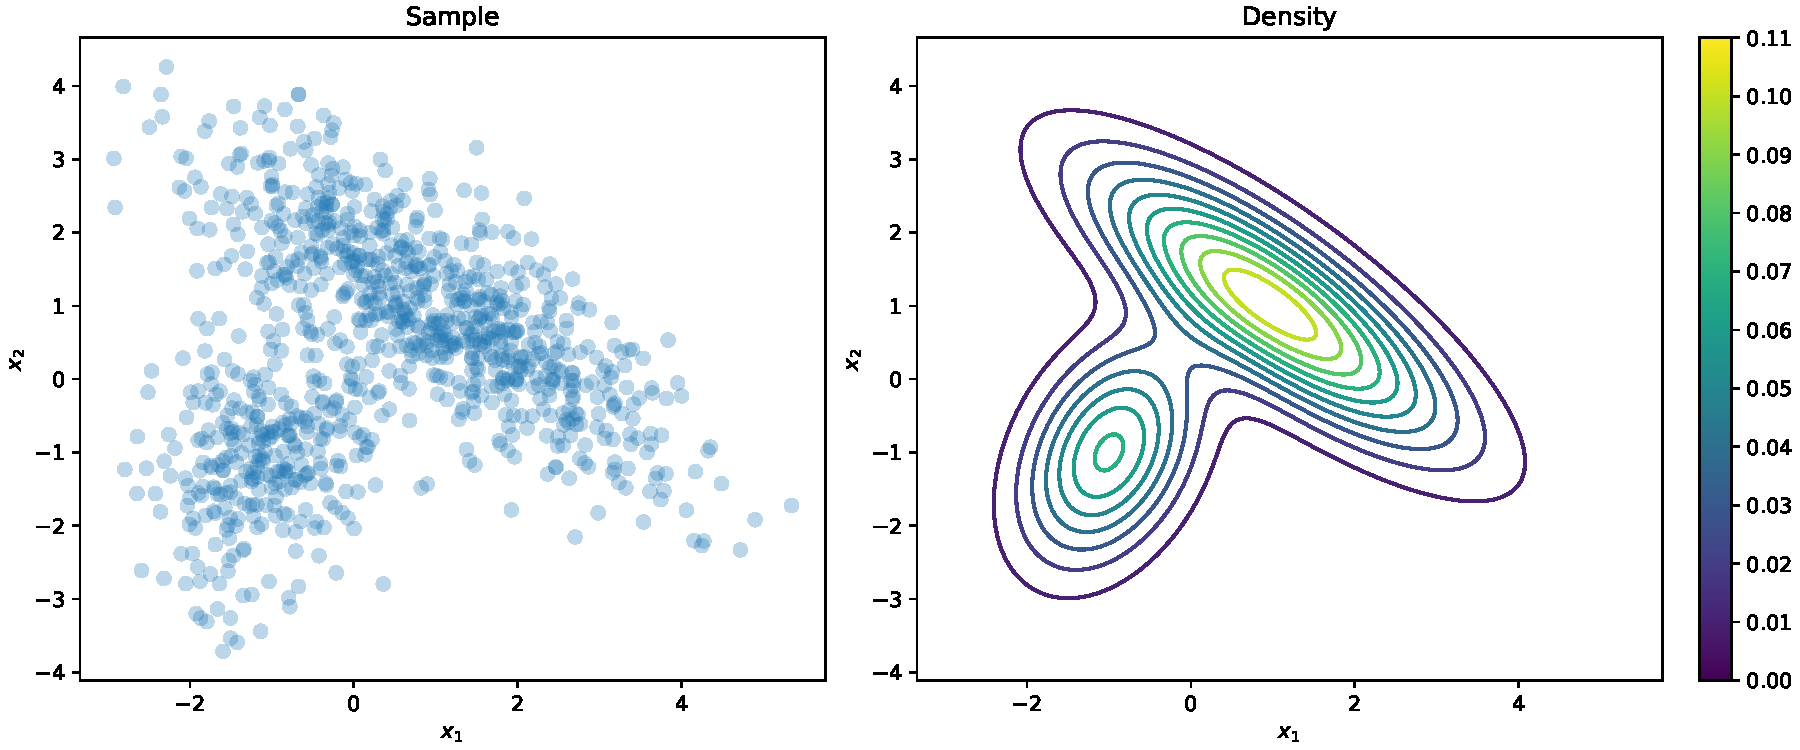
\includegraphics[width=1.0\textwidth]{gaussian-mixture-sample.pdf}
}
\end{figure}

\end{frame}

\begin{frame}
\frametitle{Bivariate Gaussian mixture: thinning approaches}

We evaluate the following approaches:
\begin{itemize}
\item na\"ive thinning,
\item standard Stein thinning,
\item gradient-free Stein thinning with different choices of $Q$:
	\begin{itemize}
	\item multivariate Gaussian using the sample mean and covariance,
	\item Laplace approximation,
	\item KDE approximation.
	\end{itemize}
\end{itemize}

\end{frame}

\begin{frame}
\frametitle{Bivariate Gaussian mixture: thinning results}

\begin{figure}[H]
\centering
\makebox[\textwidth][c]{
	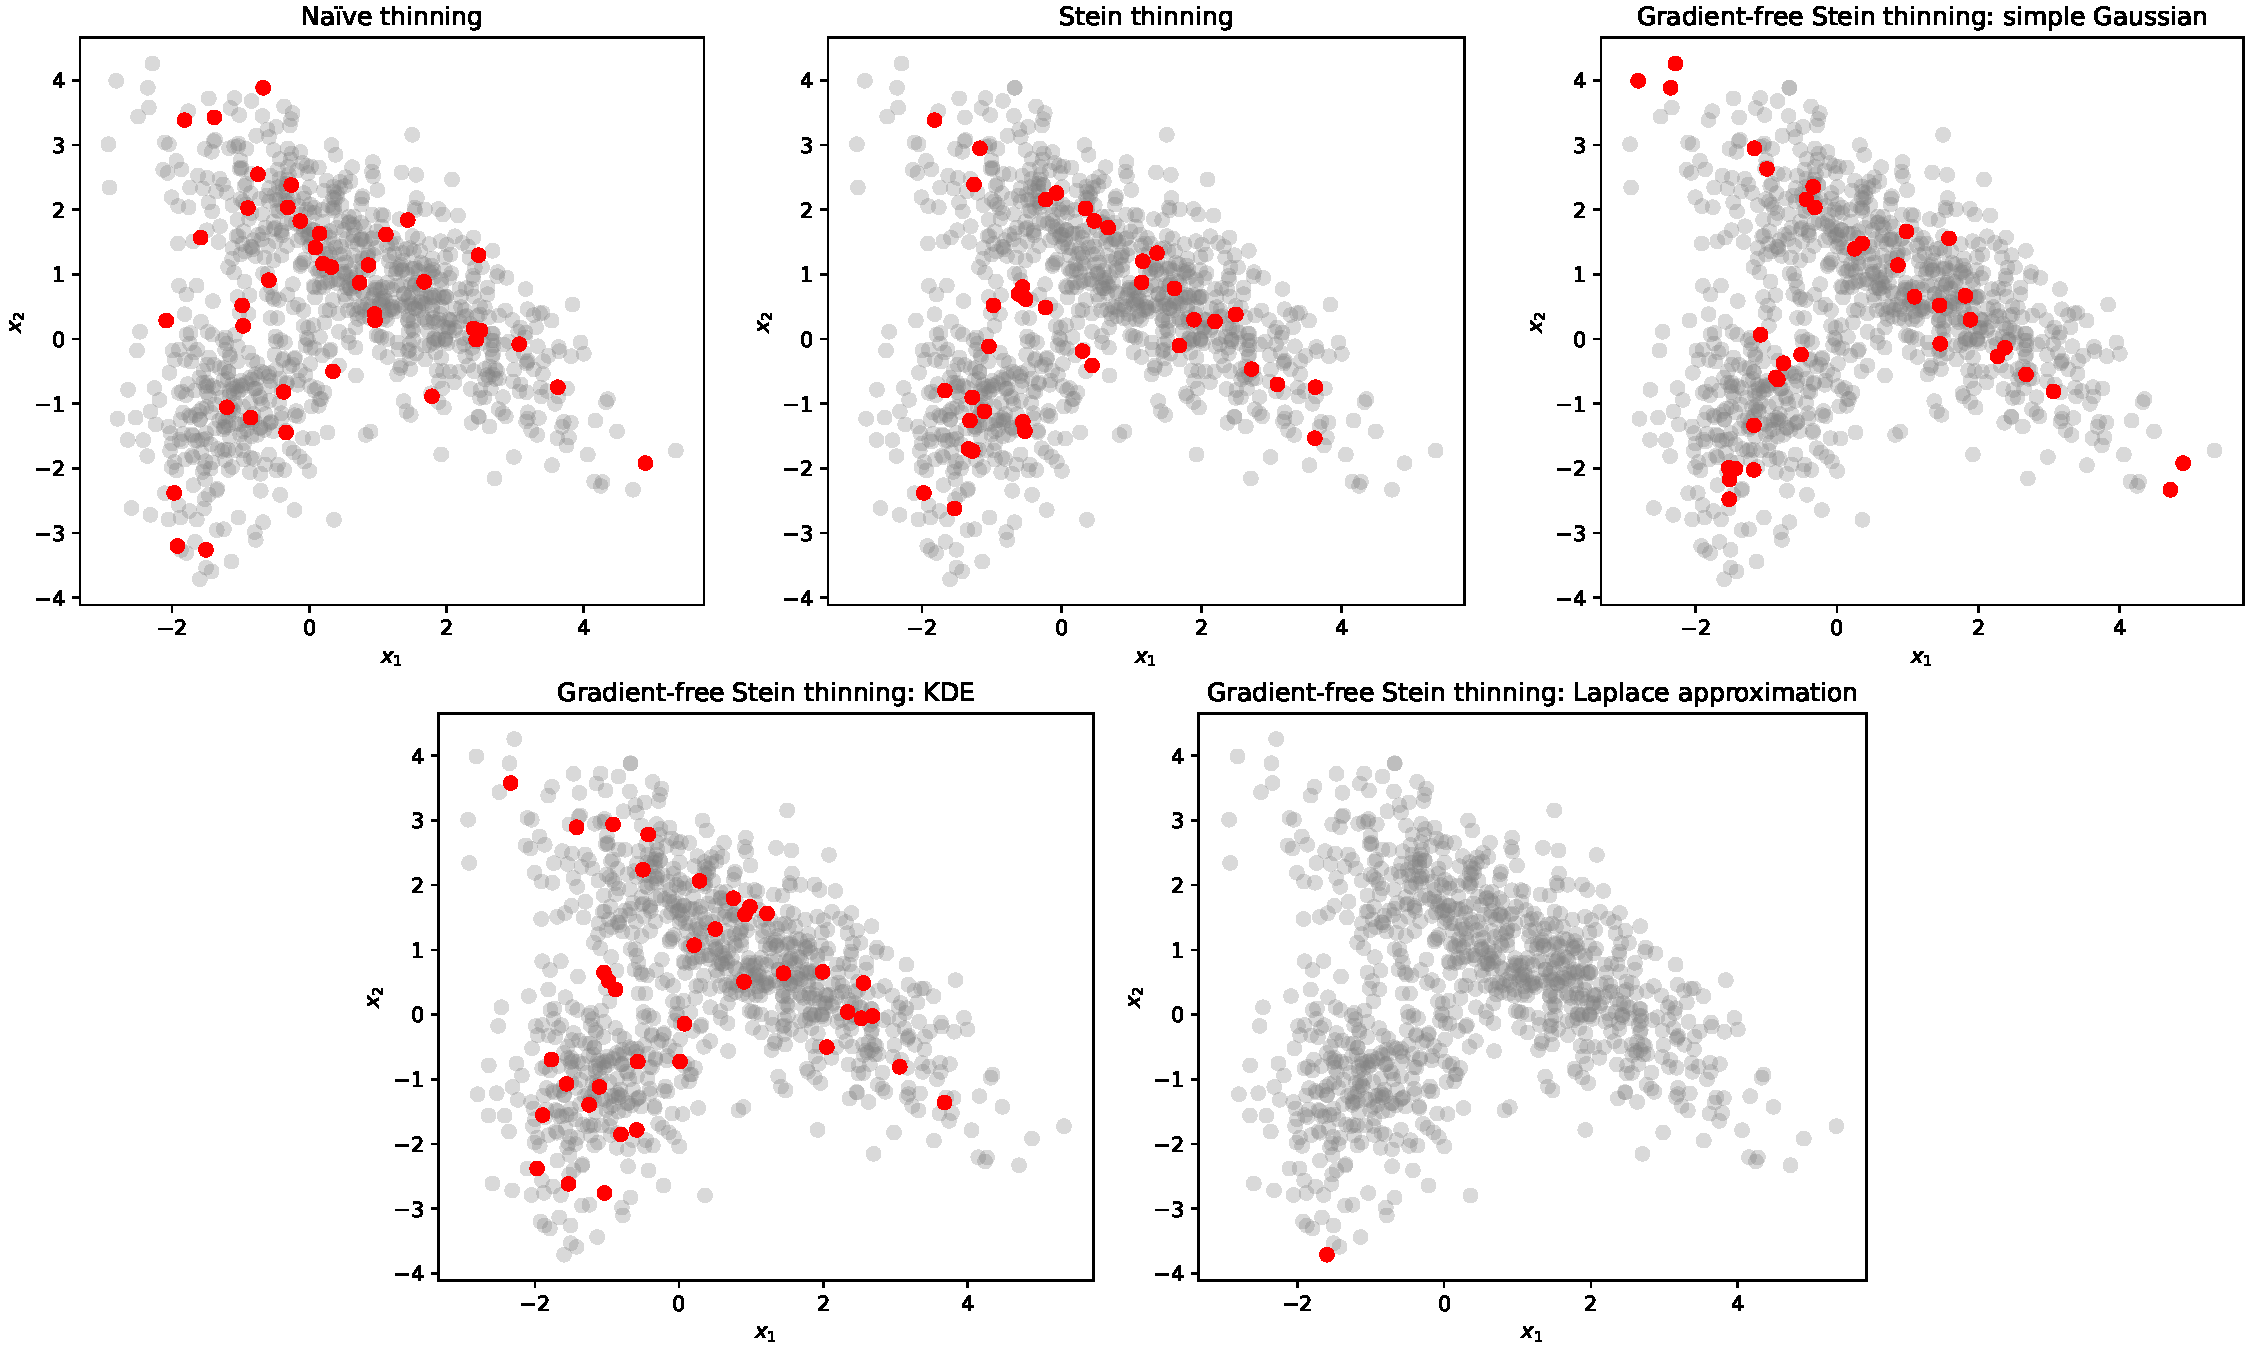
\includegraphics[width=1.0\textwidth]{gaussian-mixture-thinned-20.pdf}
}
\end{figure}

\end{frame}

\begin{frame}
\frametitle{Bivariate Gaussian mixture: comparison of approaches}

\begin{figure}[h]
\centering
\makebox[\textwidth][c]{
	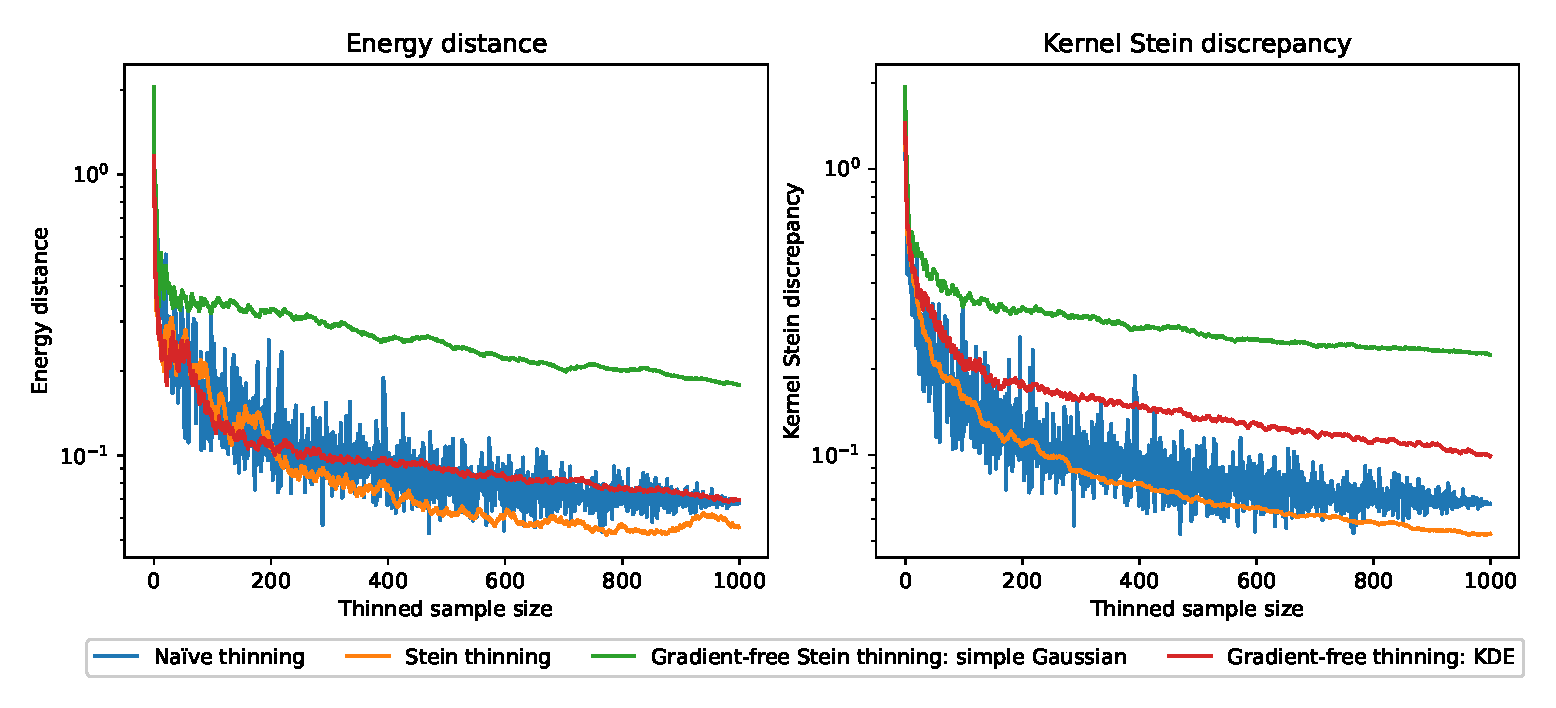
\includegraphics[width=1.0\textwidth]{gaussian-mixture-comparison.eps}
}
\end{figure}

\end{frame}

\subsection{Lotka-Volterra inverse problem}

\begin{frame}
\frametitle{Lotka-Volterra inverse problem}

The Lotka-Volterra model describes the evolution of an idealised ecosystem with two species: predator and prey.

Let $u_1$ be the size of the prey population and $u_2$ the size of the predator population. The model then postulates the following dynamic:
\begin{equation*}
\begin{aligned}
\frac{\diff u_1}{\diff t} & = \theta_1 u_1 - \theta_2 u_1 u_2, \\
\frac{\diff u_2}{\diff t} & = -\theta_3 u_2 + \theta_4 u_1 u_2, \\
\end{aligned}
\end{equation*}
with $\theta_1, \dots, \theta_4 > 0$.

The inverse problem: given a noisy realisation
\begin{equation*}
y(t) = \begin{pmatrix}
u_1(t) \\ u_2(t)
\end{pmatrix}
+ \varepsilon(t),
\end{equation*}
infer $\theta = (\theta_1, \dots, \theta_4)^T$ that best describes the observed behaviour.

\end{frame}

\begin{frame}
\frametitle{Lotka-Volterra inverse problem: synthetic data}

\begin{block}{Lotka-Volterra model}
\begin{equation*}
\begin{aligned}
\frac{\diff u_1}{\diff t} & = \theta_1 u_1 - \theta_2 u_1 u_2, \\
\frac{\diff u_2}{\diff t} & = -\theta_3 u_2 + \theta_4 u_1 u_2, \\
\end{aligned}
\end{equation*}
\end{block}

We solve the model with parameters
\begin{equation*}
\theta^* = (0.67, 1.33, 1, 1)^T
\end{equation*}
and initial values
\begin{equation*}
u(0) = (1, 1)^T
\end{equation*}
for $t \in [0, 25]$ discretised into $N = 2400$ points.

We then add bivariate i.i.d.\ Gaussian noise:
\begin{equation*}
\varepsilon(t) \sim \mathcal{N}(0, \diag(0.2^2, 0.2^2)).
\end{equation*}

\end{frame}

\begin{frame}
\frametitle{Lotka-Volterra inverse problem: synthetic data}

The resulting noisy data is used as the input for the inverse problem:

\begin{figure}[h]
\centering
\makebox[\textwidth][c]{
	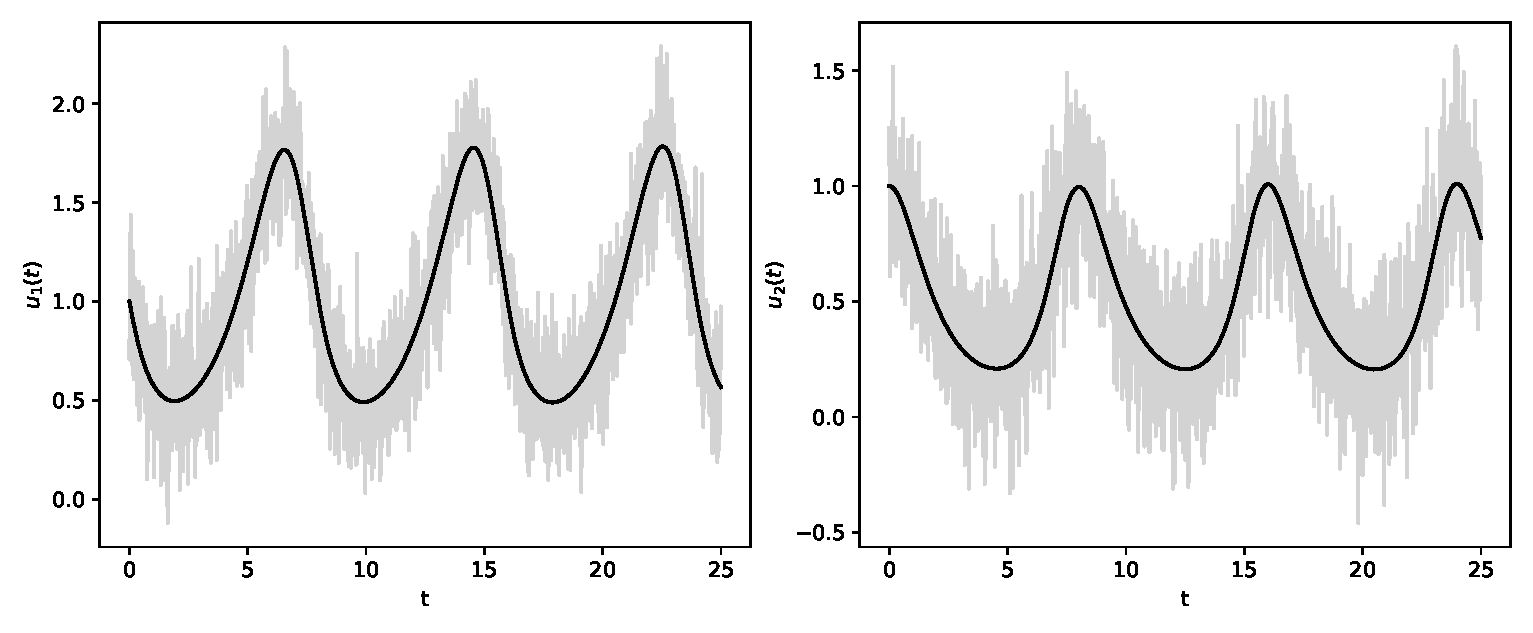
\includegraphics[width=1.0\textwidth]{lotka-volterra.eps}
}
\end{figure}

\end{frame}

\begin{frame}
\frametitle{Lotka-Volterra inverse problem: Bayesian inference}

Assuming independent observations, we take the likelihood to be
\begin{equation*}
\mathcal{L}(\theta) = \prod_{i=1}^N \phi_i(u(t_i; \theta)),
\end{equation*}
where 
\begin{equation*}
\phi_i(u(t_i;\theta)) \propto \exp\left( -\frac{1}{2} (y(t_i) - u(t_i; \theta))^T C^{-1} (y(t_i) - u(t_i; \theta)) \right)
\end{equation*}
with $C = \diag(0.2^2, 0.2^2)$.

Since $\theta_k > 0$, we put independent log-normal priors on each $\theta_k$:
\begin{equation*}
\pi(\theta) \propto \exp \left(-\frac{1}{2} (\log \theta)^T (\log \theta) \right).
\end{equation*}

By the Bayes theorem, the posterior is then
\begin{equation*}
p(\theta) \propto \mathcal{L}(\theta) \pi(\theta).
\end{equation*}

\end{frame}

\begin{frame}
\frametitle{Lotka-Volterra inverse problem: MCMC}

The inference is performed using the Metropolis-Hastings algorithm with the starting points taken from \cite{riabizOptimalThinningMCMC2022}:

\begin{table}[H]
\centering
\begin{tabularx}{0.5\textwidth}{c Y Y Y Y} 
 \hline
 Chain & $\theta_1$ & $\theta_2$ & $\theta_3$ & $\theta_4$ \\
 \hline
 1 & 0.55 & 1    & 0.8 & 0.8 \\ 
 2 & 1.5  & 1    & 0.8 & 0.8 \\
 3 & 1.3  & 1.33 & 0.5 & 0.8 \\
 4 & 0.55 & 3    & 3.  & 0.8 \\
 5 & 0.55 & 1    & 1.5 & 1.5 \\
 \hline
\end{tabularx}
\end{table}

Since the parameters $\theta_k$ of the Lotka-Volterra model are positive, we run MCMC in the log-space by applying the reparameterisation $\zeta_k = \log \theta_k$. 

We run 500,000 iterations of the algorithm for each chain.

\end{frame}

\begin{frame}
\frametitle{Lotka-Volterra inverse problem: MCMC sample}

The sample from the first chain is shown here for illustration:

\begin{figure}[h]
\centering
\makebox[\textwidth][c]{
	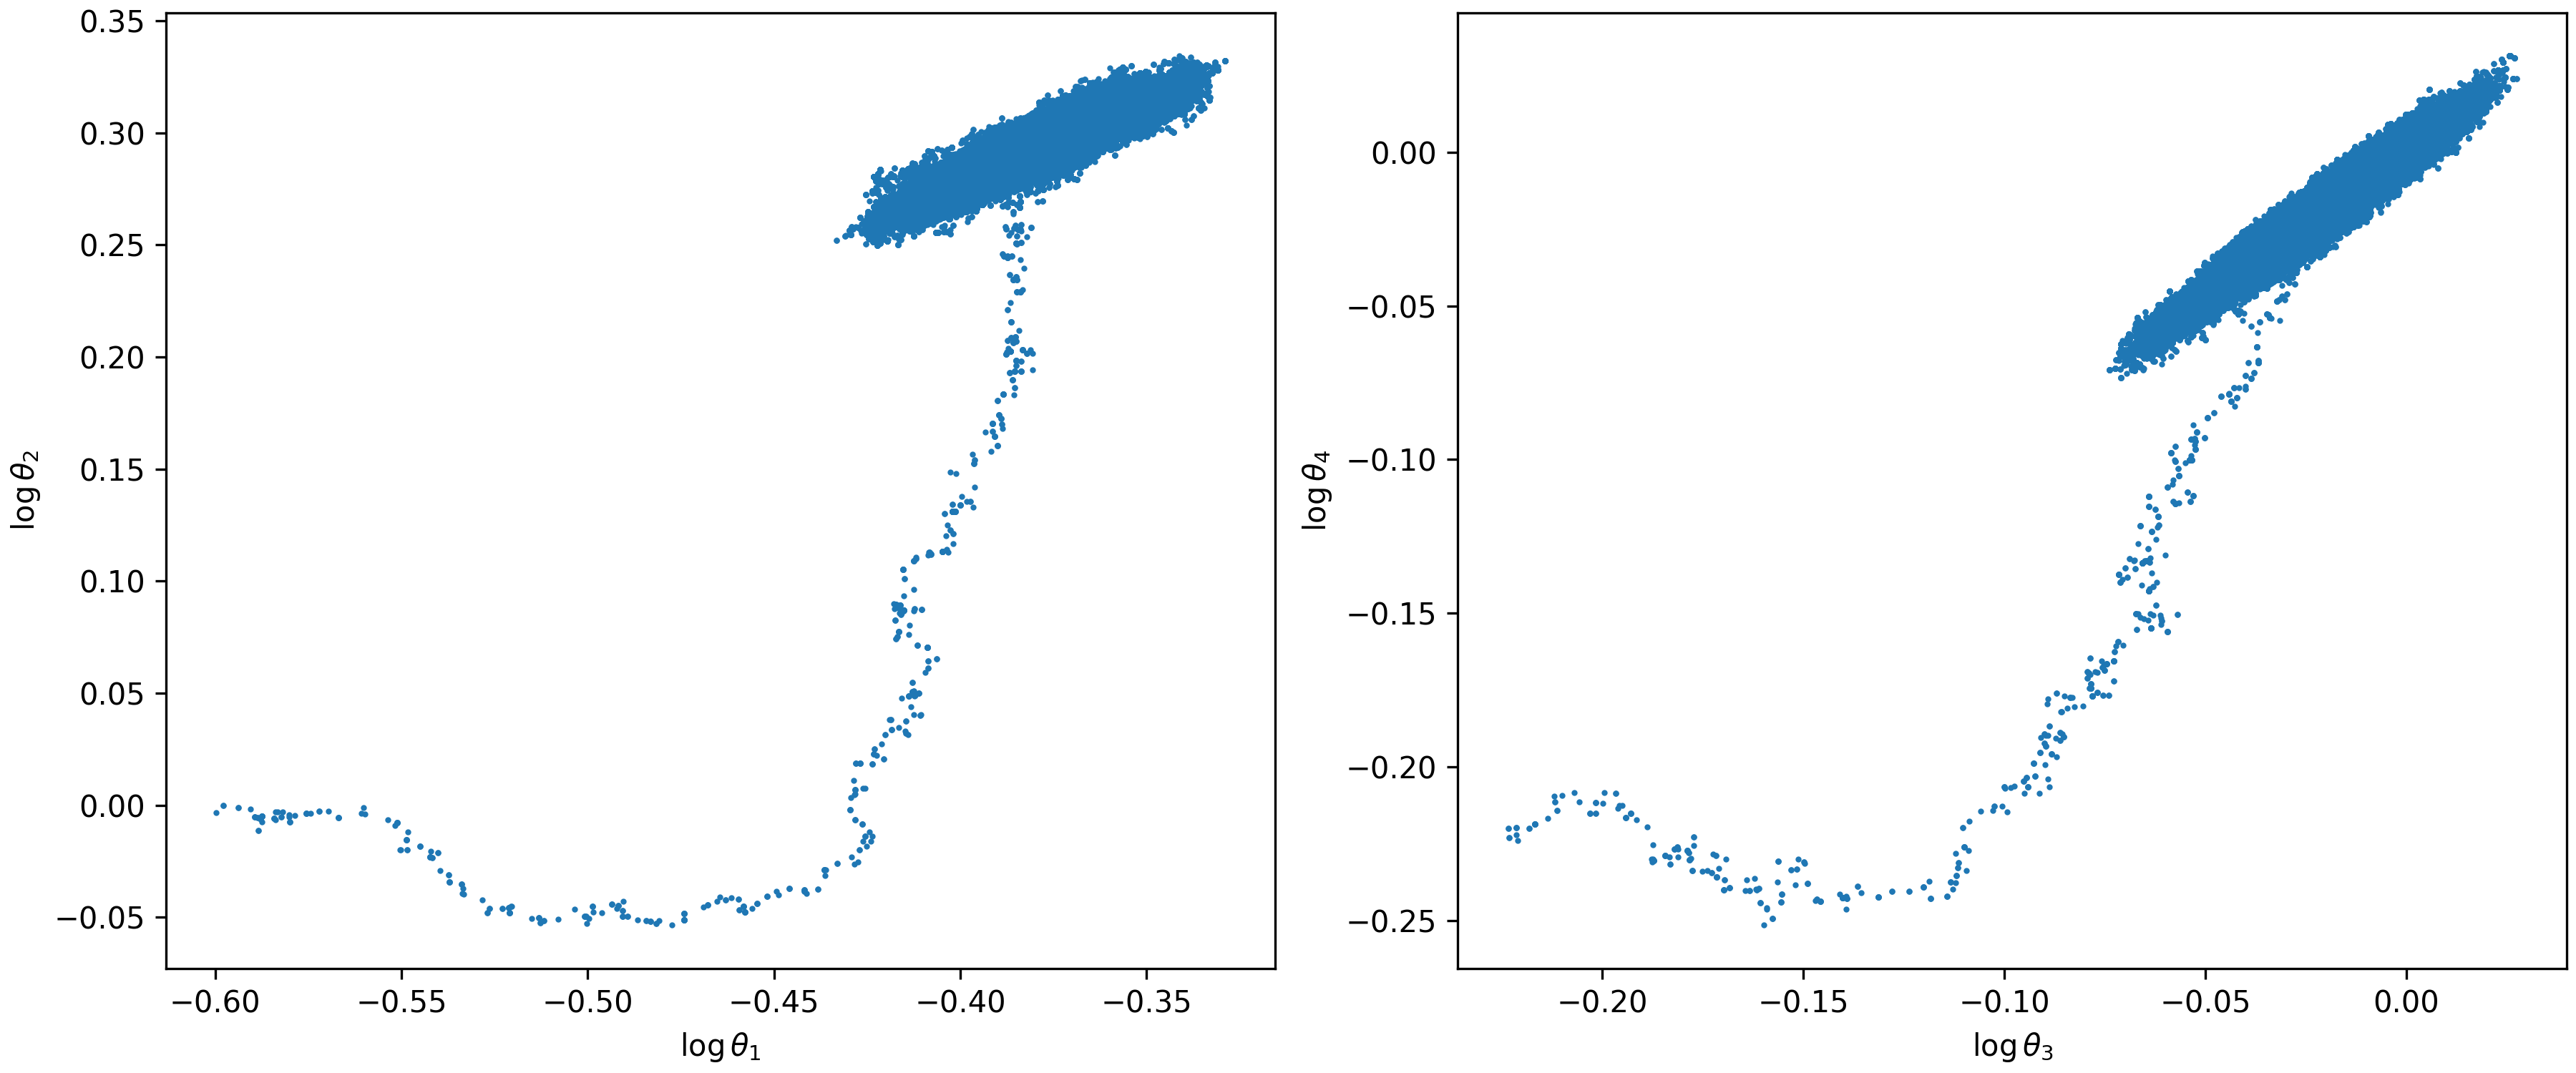
\includegraphics[width=1.0\textwidth]{lotka-volterra-chain1-sample.png}
}
\end{figure}

\end{frame}

\begin{frame}
\frametitle{Lotka-Volterra inverse problem: thinning approaches}

We evaluate the following approaches:
\begin{itemize}
\item na\"ive thinning,
\item standard Stein thinning,
\item gradient-free Stein thinning with different choices of $Q$:
	\begin{itemize}
	\item multivariate Gaussian using the sample mean and covariance,
	\item Laplace approximation - \alert{fails as in bivariate Gaussian case},
	\item KDE approximation - \alert{computationally infeasible}.
	\end{itemize}
\end{itemize}

\end{frame}

\begin{frame}
\frametitle{Lotka-Volterra inverse problem: Stein thinning}

We have a choice of applying thinning in linear or logarithmic space, however the energy distance comparison indicates no discernible difference, so we proceed to use the logarithmic space.

\begin{figure}[h]
\centering
\makebox[\textwidth][c]{
	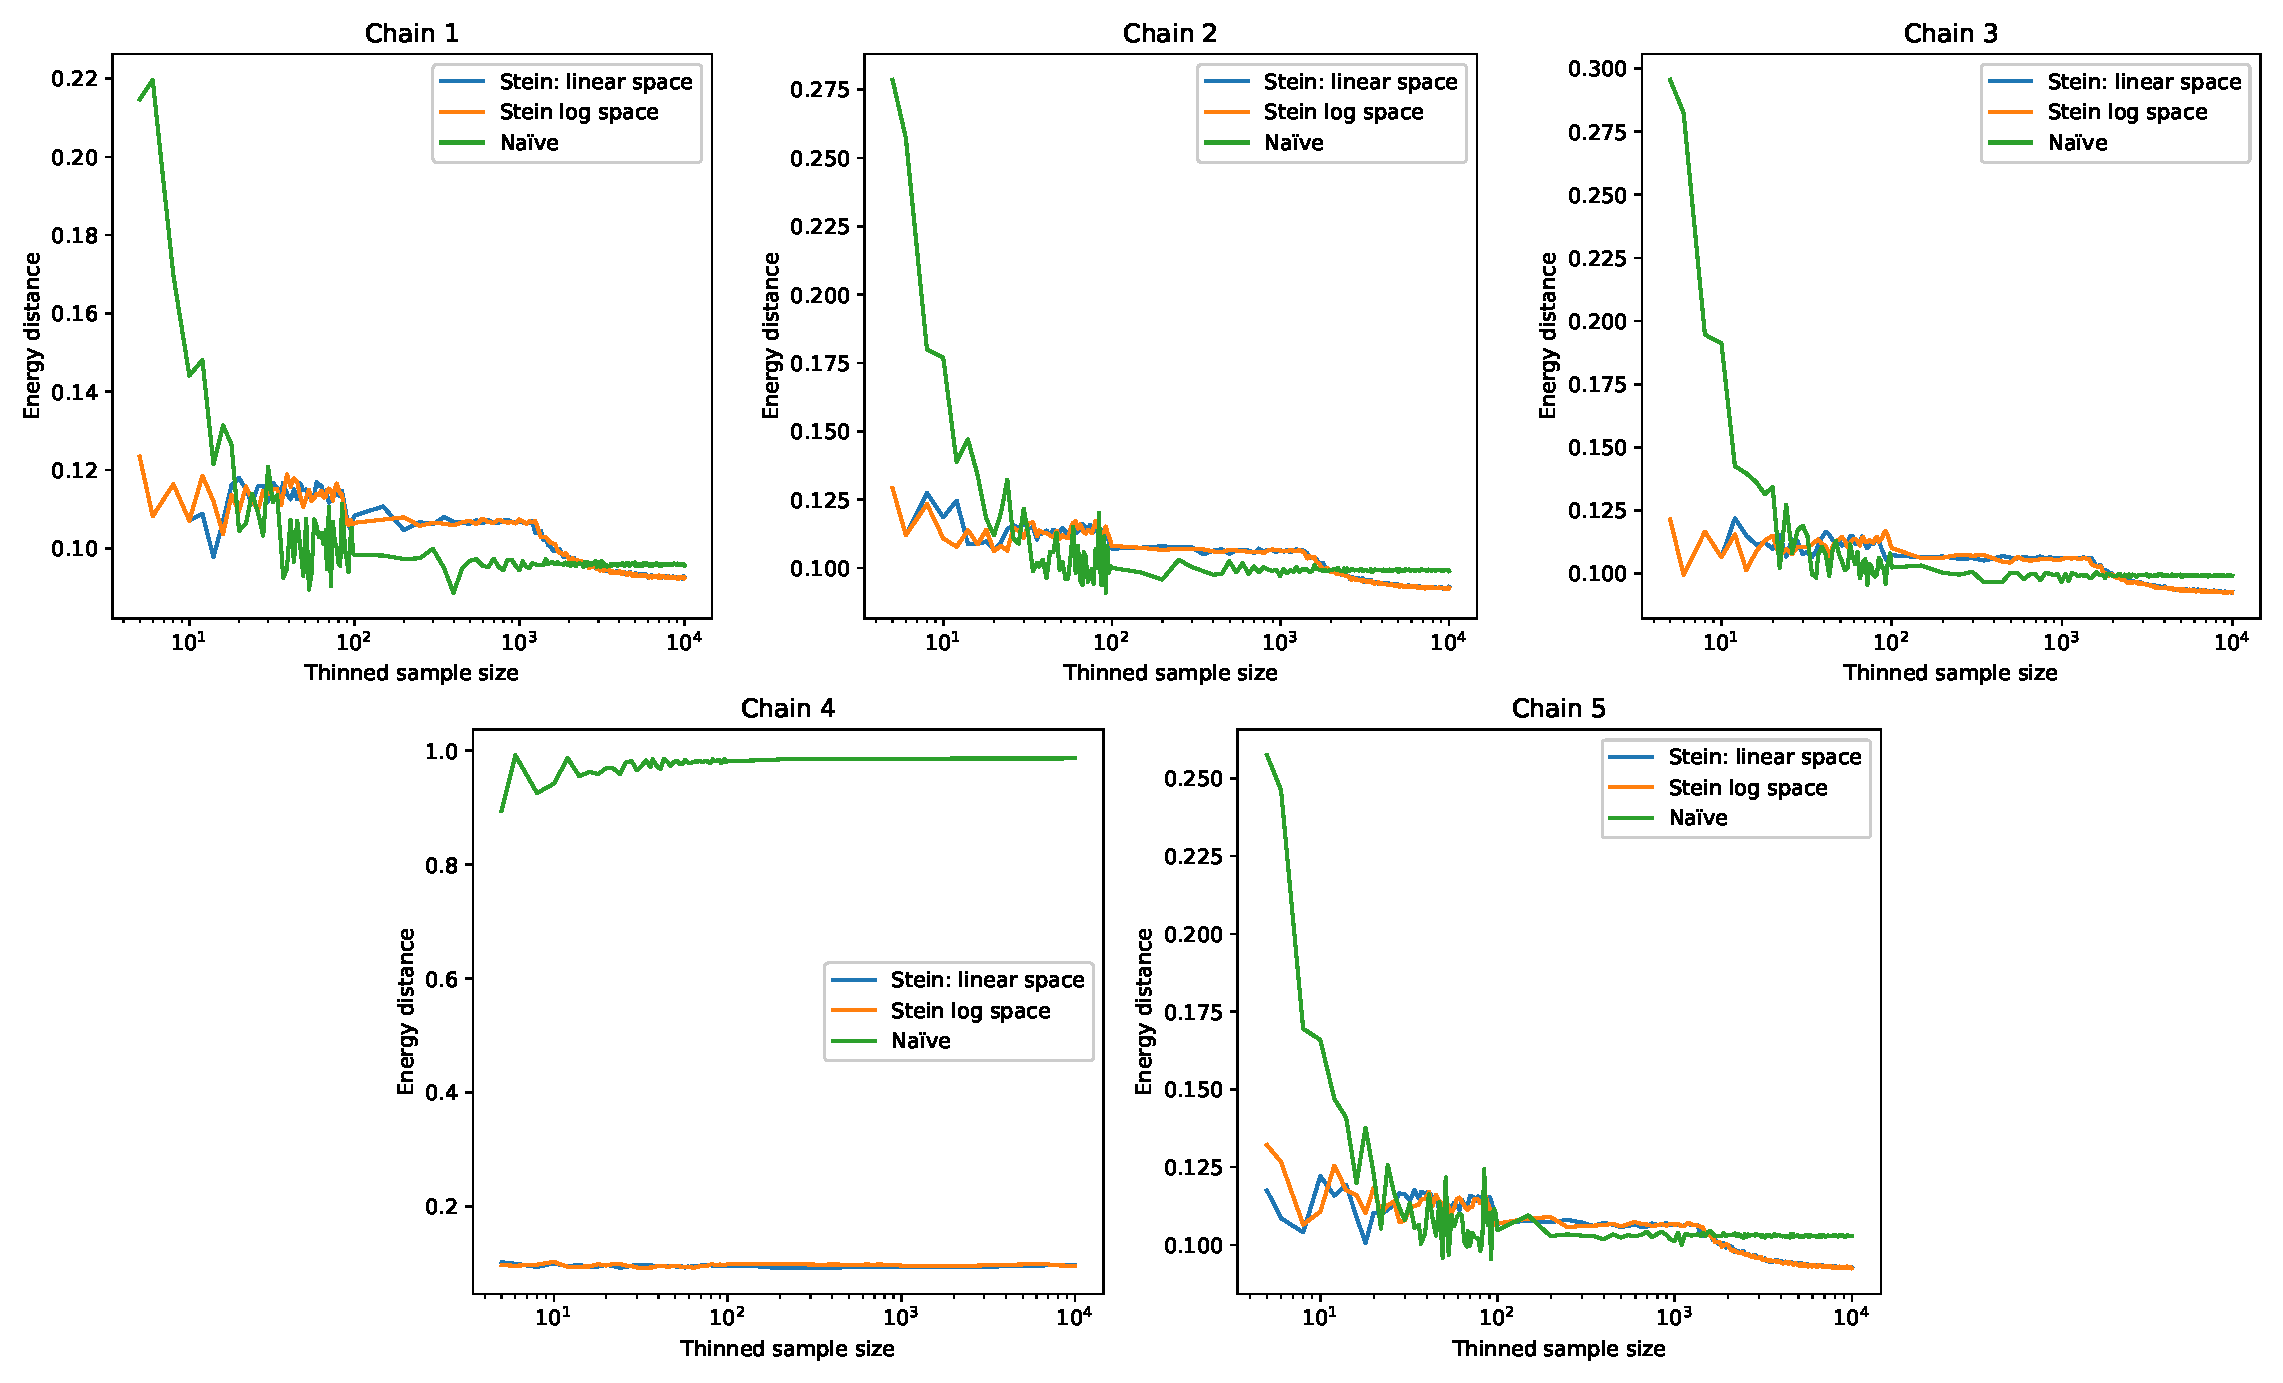
\includegraphics[width=0.8\textwidth]{lotka-volterra-stein-thinning-energy-distance.eps}
}
\end{figure}

\end{frame}

\begin{frame}
\frametitle{Lotka-Volterra inverse problem: comparison of approaches}

Gradient-free thinning using a multivariate Gaussian with the sample mean and covariance matrix performs comparably with the gradient-based approach, notably for chain 4, when compared using the energy distance:

\begin{figure}[h]
\centering
\makebox[\textwidth][c]{
	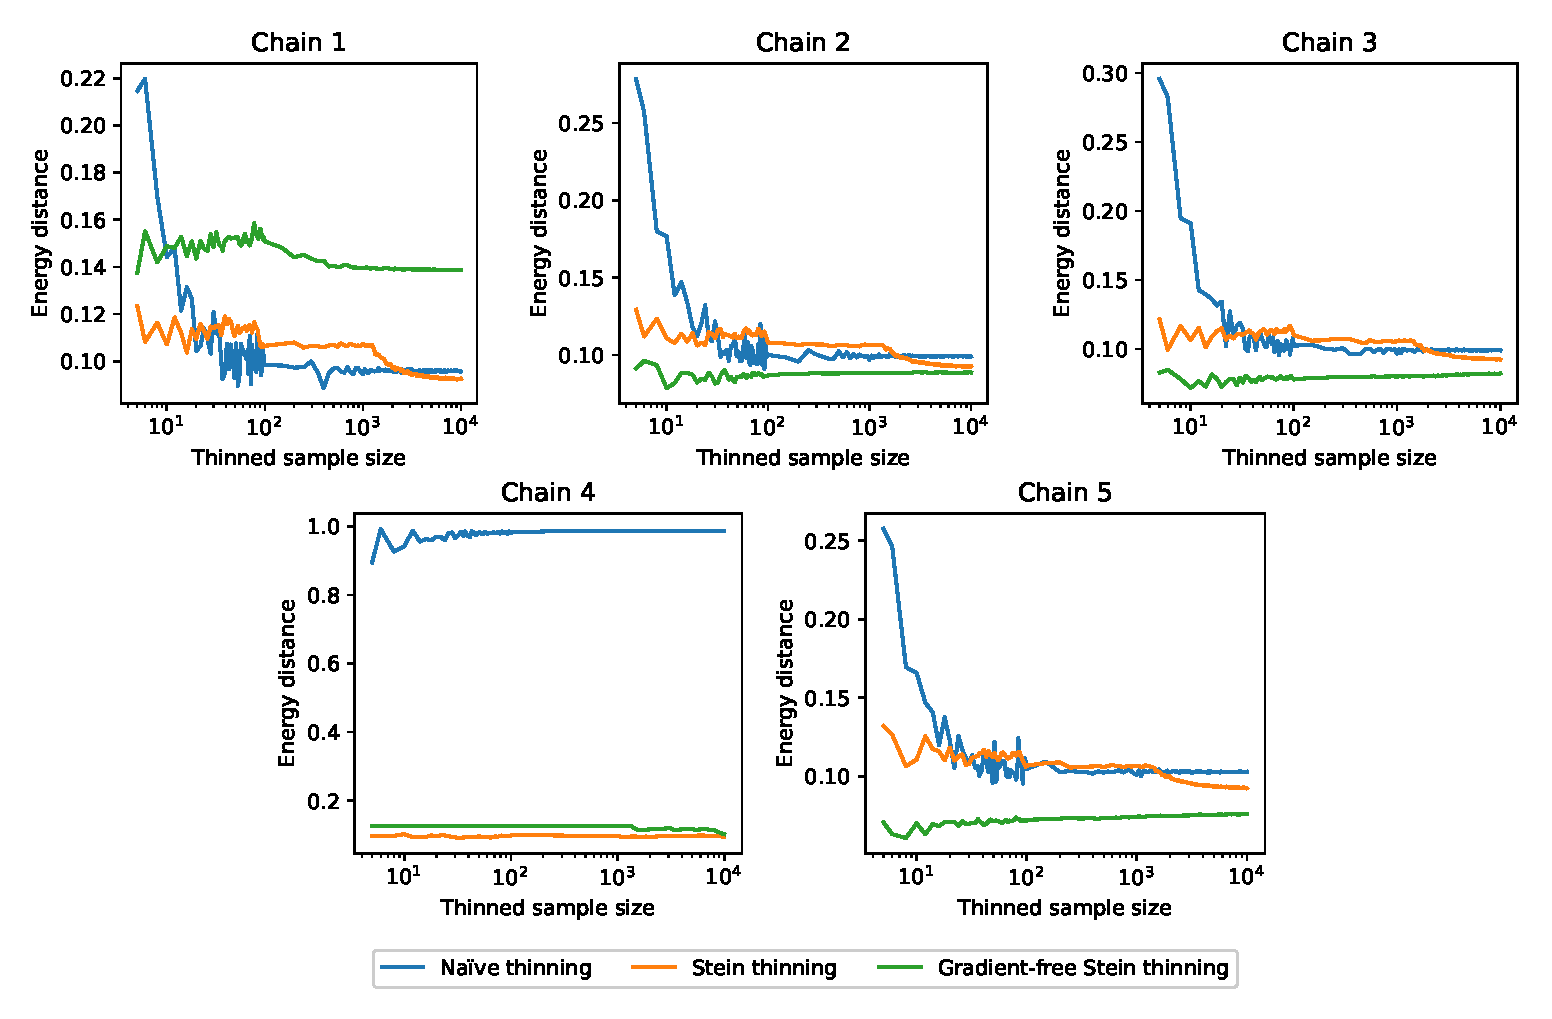
\includegraphics[width=0.8\textwidth]{lotka-volterra-gf-thinning-energy-distance.eps}
}
\end{figure}

\end{frame}

\begin{frame}
\frametitle{Lotka-Volterra inverse problem: comparison of approaches}

Gradient-free thinning offers a significant improvement over na\"ive thinning in terms of KSD:

\begin{figure}[h]
\centering
\makebox[\textwidth][c]{
	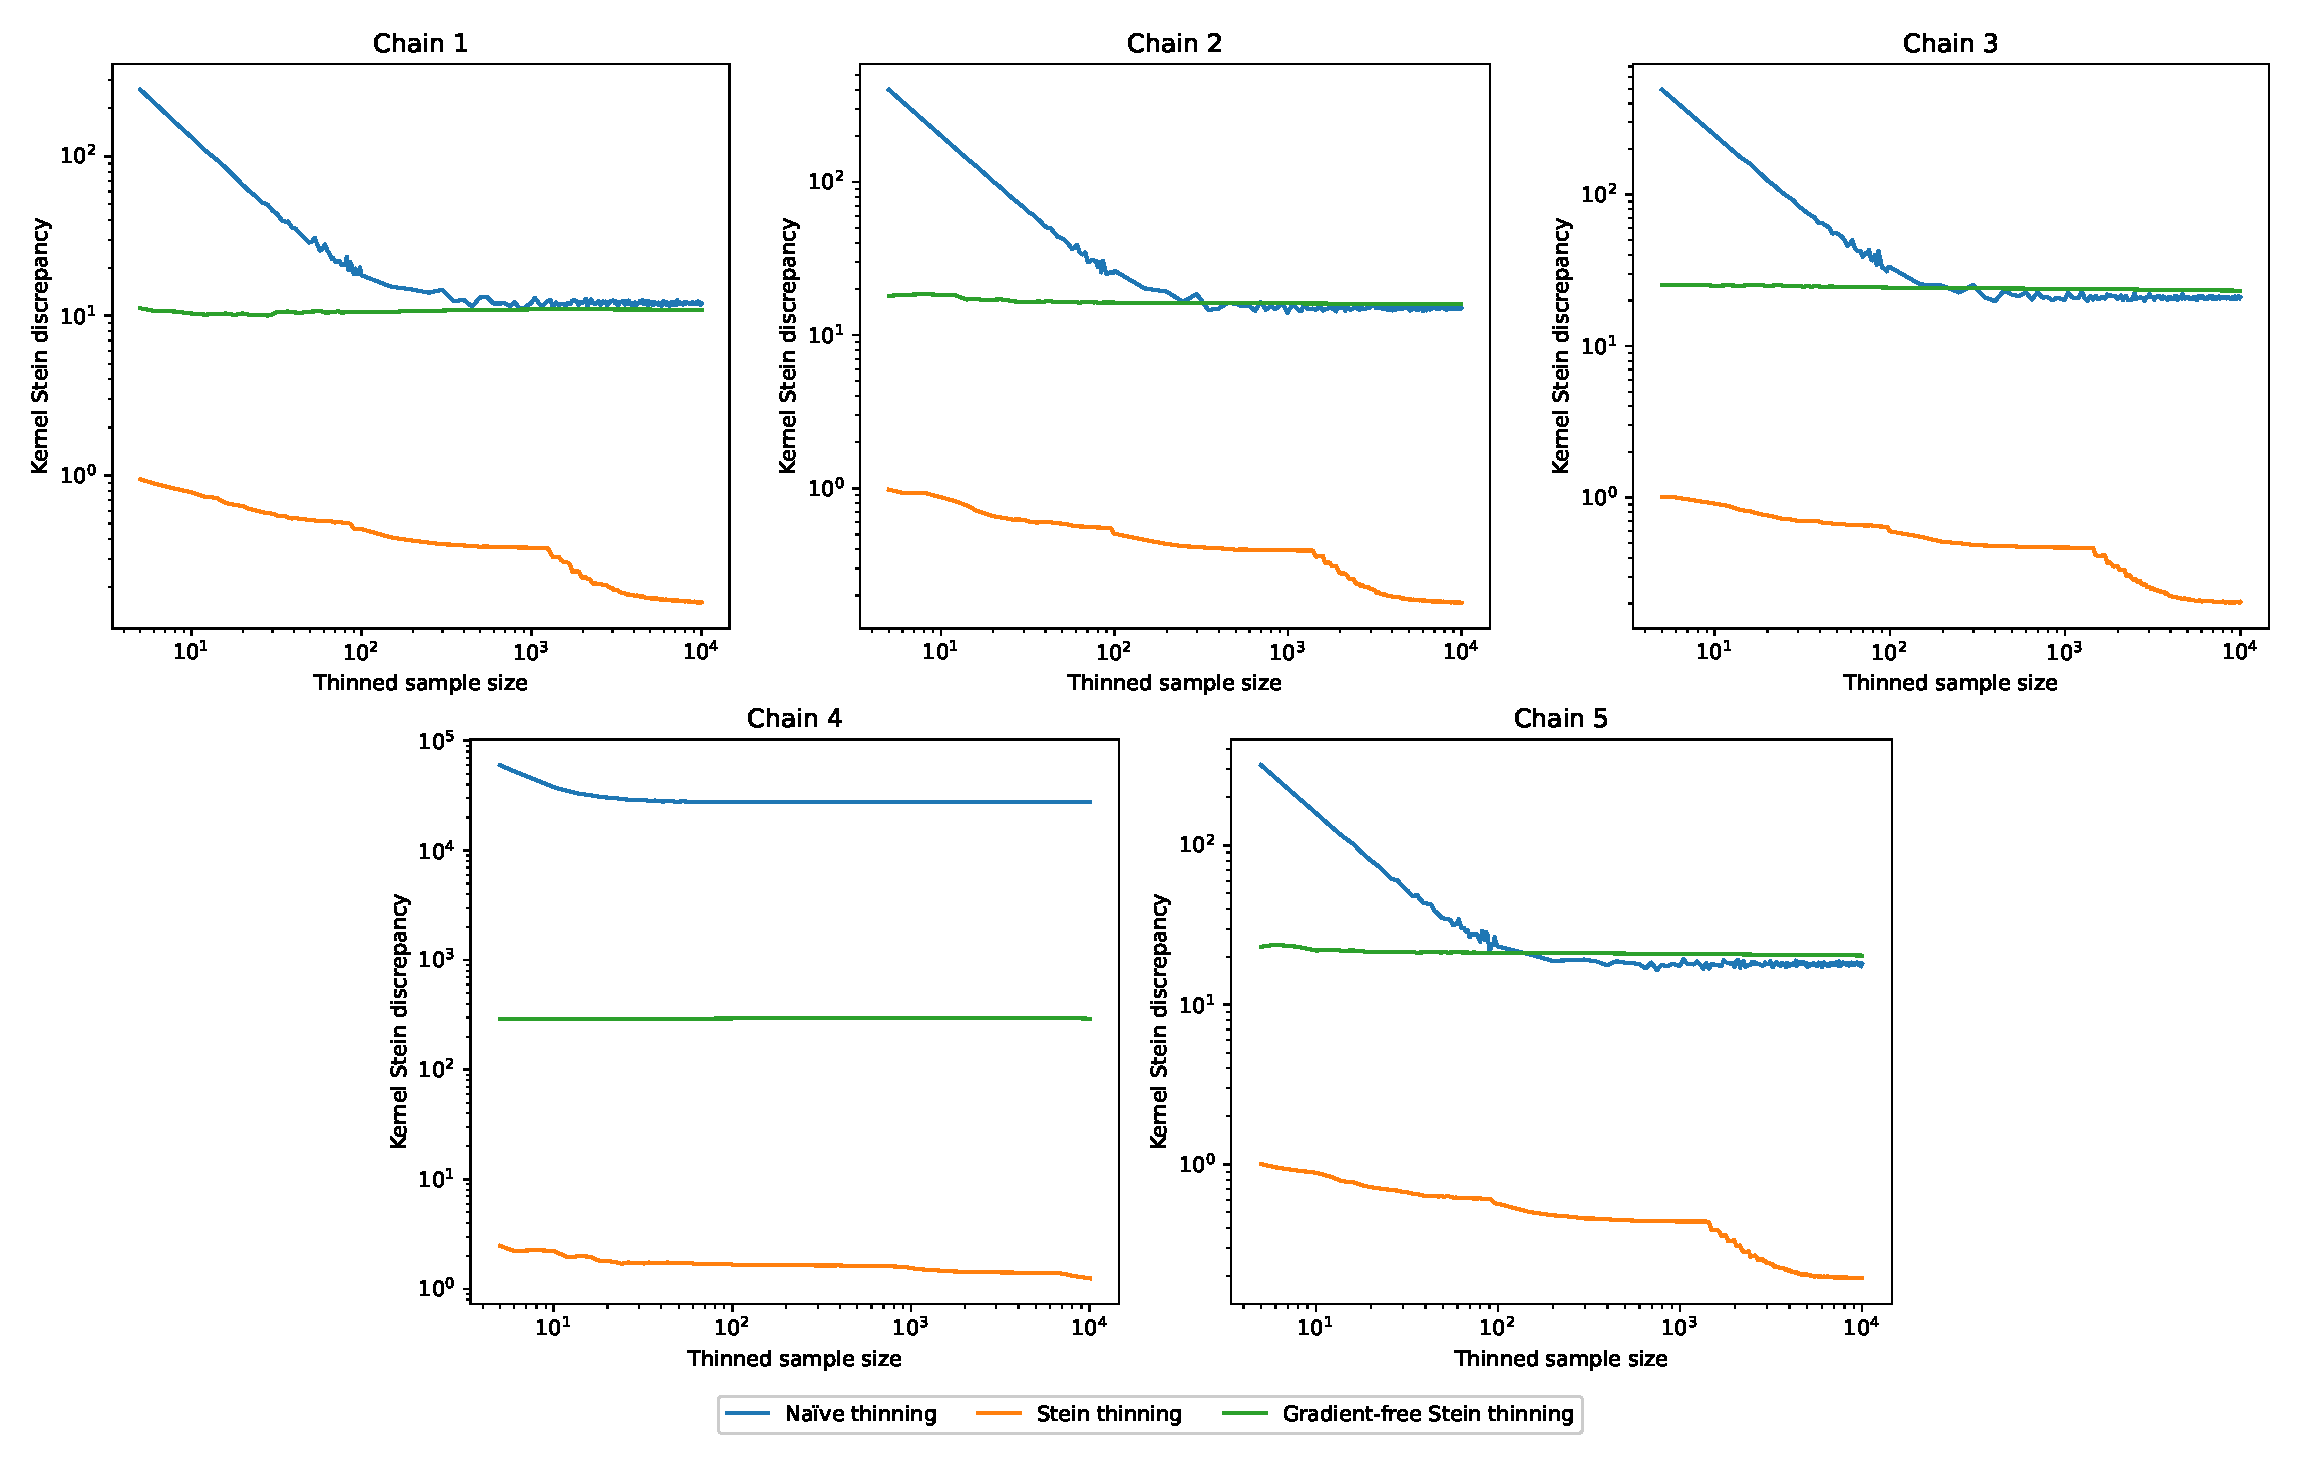
\includegraphics[width=0.8\textwidth]{lotka-volterra-gf-thinning-ksd.eps}
}
\end{figure}

\end{frame}

\section{Conclusions}

\begin{frame}
\frametitle{Contribution}

The project makes three contributions:
\begin{itemize}
\item implementation of the gradient-free Stein thinning algorithm in the Python library \texttt{stein-thinning},
\item evaluation of the performance of the proposed algorithm,
\item improvement of the computational efficiency of the existing Stein thinning algorithm from $O(nm^2)$ to $O(nm)$, where $n$ is the input sample size and $m$ is the desired thinned sample size.
\end{itemize}

\end{frame}

\begin{frame}
\frametitle{Conclusions}

\begin{itemize}
\item The gradient-free approach is feasible and performs similarly to the Stein thinning algorithm of \cite{riabizOptimalThinningMCMC2022} for small thinned sample sizes,
\item The performance of the algorithm depends crucially on the choice of the auxiliary distribution. For example, even in the highly favourable setting of i.i.d.\ samples from a Gaussian mixture, choosing the auxiliary distribution based on the Laplace approximation fails to produce a thinned sample.
\item The simple multivariate Gaussian distribution using the sample mean and covariance offered a good starting point in our experiments, however bespoke treatment might be required for more complex problems.
\item In deciding whether to use the new algorithm as opposed to the gradient-based approach, the effort involved in selecting a good auxiliary distribution must be weighed against the computational cost of obtaining gradients.
\end{itemize}

\end{frame}

\section{Further Research}

\begin{frame}
\frametitle{Further Research}
\begin{itemize}

\item Evaluate the choices of KDE kernels other than Gaussian for constructing the auxiliary distribution.

\item Parallelise the computation of KDE.

\item Perform thinning in a lower-dimensional space.

\item Investigate the behaviour of Stein thinning for large thinned sample sizes.

\item Compare the performance of the approaches in terms of estimating the true parameters of the Lotka-Volterra model.

\item Run an experiment with randomised starting points.

\end{itemize}

\end{frame}

\begin{frame}
\frametitle{Further Research (continued)}

\begin{itemize}

\item Repeat the experiments with more advanced MCMC algorithms. 

\item Check how running a gradient-free MCMC sampling algorithm (such the random-walk Metropolis-Hastings) followed by Stein thinning of the sample compares to running a gradient-based sampling algorithm (e.g. HMC).

\item Provide theoretical justification for gradient-free Stein thinning.

\item Explore other gradient-free alternatives.

\end{itemize}

\end{frame}

\section{References}

\begin{frame}[allowframebreaks]
\frametitle{References}

\fontsize{10pt}{12}\selectfont

\bibliographystyle{../report/plainnat_modified}
\bibliography{../report/biblio}

\end{frame}

\end{document}